\documentclass[12pt]{article}
\usepackage[margin=1.2in]{geometry}
\usepackage{tikz}
\usetikzlibrary{arrows}
\tikzset{>=latex}
\usepackage{amsmath,amsfonts,amssymb}
\renewcommand{\baselinestretch}{1.4}
\setlength\parindent{0pt}
\everymath{\displaystyle}
\begin{document}
\centerline{\fbox{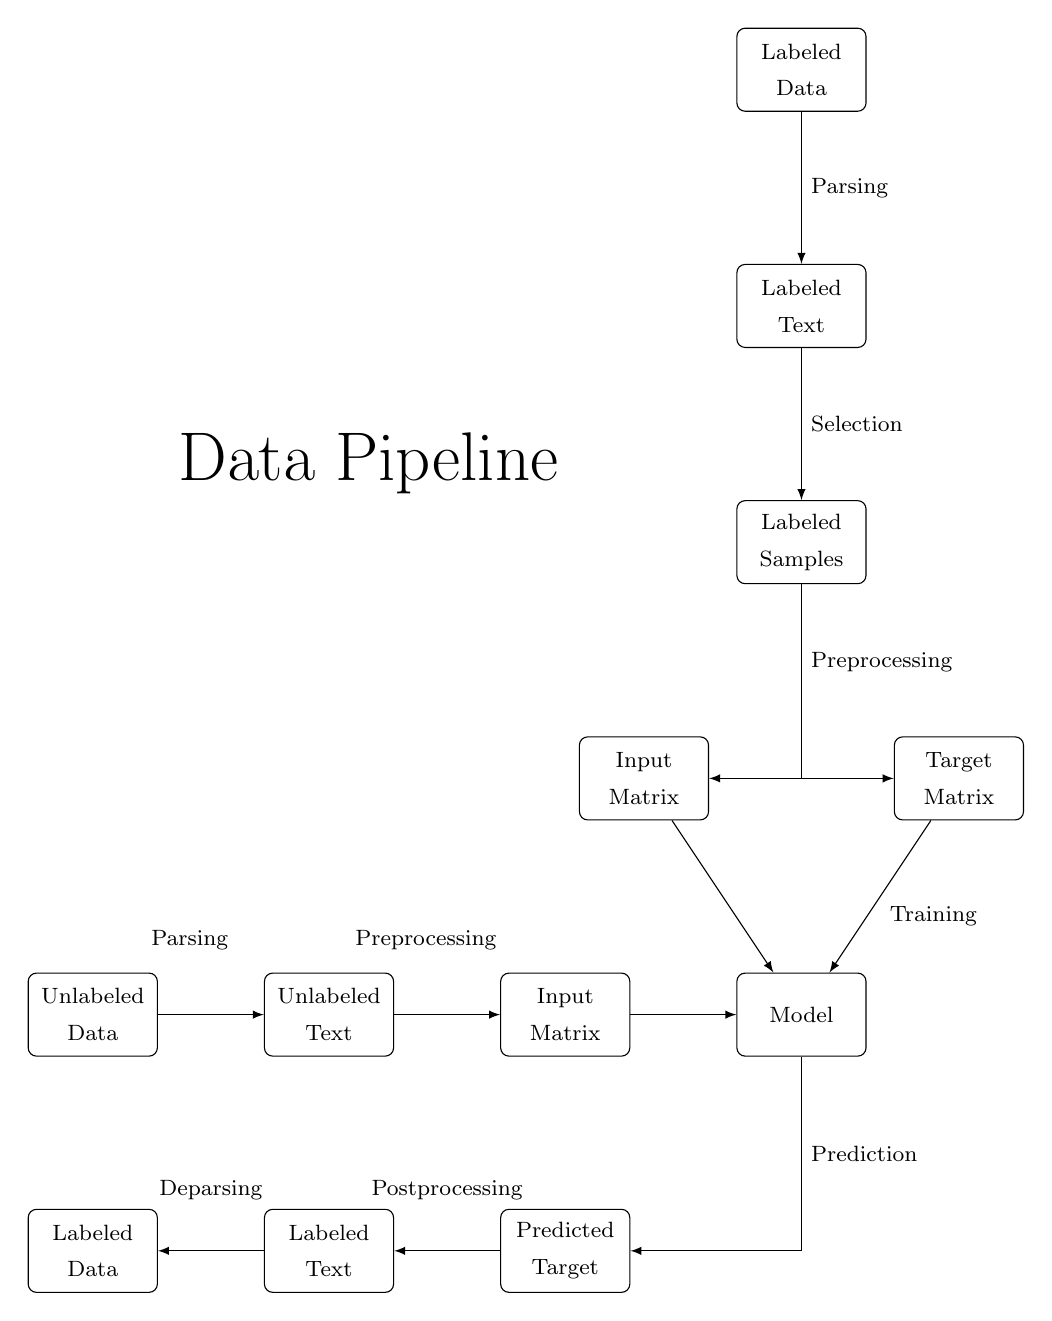
\begin{tikzpicture}[->,auto,align=center]
\tikzstyle{obj} = [font=\footnotesize,rectangle,draw,align=center, text width=4em, minimum height = 3em,rounded corners=3pt]
\node at (-5.5, 7) {\Huge Data Pipeline};
\node[obj] (raw) at (0,12) {Labeled Data};
\node[obj] (pars) at (0,9) {Labeled Text};
\node[obj] (sel) at (0,6) {Labeled Samples};
\node[obj] (in) at (-2,3) {Input Matrix};
\node[obj] (targ) at (2,3) {Target Matrix};
\node[obj] (mod) at (0,0) {Model};
\node[obj] (uraw) at (-9,0) {Unlabeled Data};
\node[obj] (upars) at (-6,0) {Unlabeled Text};\\
\node[obj] (uin) at (-3,0) {Input Matrix};
\node[obj] (utarg) at (-3,-3) {Predicted Target};
\node[obj] (ulpars) at (-6,-3) {Labeled Text};
\node[obj] (ulraw) at (-9,-3) {Labeled Data};
\draw (raw) -> (pars) node[pos=0.5] {\footnotesize Parsing};
\draw (pars) -> (sel) node[pos=0.5] {\footnotesize Selection};
\draw (sel) |- (in);
\draw (sel) |- (targ) node[pos=0.2] {\footnotesize Preprocessing};
\draw (in) -> (mod);
\draw (targ) -> (mod) node[pos=0.5] {\footnotesize Training};
\draw (uraw) -> (upars) node[pos=0.3,above=2em] {\footnotesize Parsing};
\draw (upars) -> (uin) node[pos=0.3,above=2em] {\footnotesize Preprocessing};
\draw (uin) -> (mod);
\draw (mod) |- (utarg) node[pos=0.25] {\footnotesize Prediction};
\draw (utarg) -> (ulpars) node[pos=0.5,above=1.5em] {\footnotesize Postprocessing};
\draw (ulpars) -> (ulraw) node[pos=0.5,above=1.5em] {\footnotesize Deparsing};
\end{tikzpicture}}}
\end{document}